%%%%%%%%%%%%%%%%%%%%%%%%%%%%%%%%%%%%%%%%%%%%%%%%%%%%%%%%%%%%%%%%%%%%%%%%%%%%%
\section{Hybrid MPI+Threads Programming}\label{sec:back-hybrid}
%%%%%%%%%%%%%%%%%%%%%%%%%%%%%%%%%%%%%%%%%%%%%%%%%%%%%%%%%%%%%%%%%%%%%%%%%%%%%

Although the number of cores is rapidly increasing on modern multi-
and many-core architectures, the other system resources (e.g., memory,
network endpoints) are not growing at the same rate. To efficiently utilize such
large amount of threads with better resource sharing, application programmers
are increasingly looking at the hybrid MPI + Thread model, where multiple threads
are used to parallelize the computation on each computing node and MPI
is used for the inter-node data communication. The most prominent of the
threading models used in modern scientific computing is OpenMP~\cite{openmp},
where applications add annotations in the code with necessary information of
the parallelism (e.g., the number of threads, the parallel patterns and
the property of variables), then the compiler can translate these annotations
into appropriate commands and cooperate with the runtime system for task
scheduling. In the rest of this section, we focus on the MPI+OpenMP programming.

Since MPI processes and threads are managed by two separate runtime systems,
additional rules have to be made to ensure the thread safety inside MPI without
resulting in unnecessary overhead. For example, a message may be concurrently
matched by the receive calls from two threads on the same process if the
appropriate thread safety is not provided; conversely, we should also avoid
over-definition of the thread safety since it can result in significant
overhead from heavy usage of memory barriers and lock acquiring\slash releasing
in most MPI implementations even the program does not involve any threads~\cite{thread-safety}.

In this section we introduce the different threading modes defined by MPI for
multithreaded environments. The MPI standard provides four levels of thread
safety.

% \begin{figure}[ht]
%   % \vspace{-1.0ex}
%   \hspace{0.05\columnwidth}
%   \subfigure[FUNNELED.] {
%     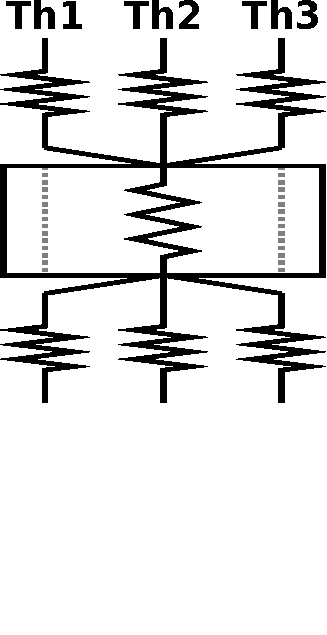
\includegraphics[width=0.26\columnwidth]{figures/mtmpi/th_funneled.pdf}
%     \label{fig:th_mode_funneled}
%   }
%   \hspace{1.0ex}
%   \subfigure[SERIALIZED.] {
%     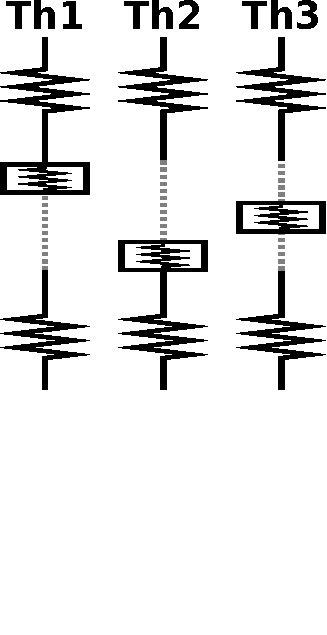
\includegraphics[width=0.26\columnwidth]{figures/mtmpi/th_serialized.pdf}
%     \label{fig:th_mode_serialized}
%   }
%   \hspace{1.0ex}
%   \subfigure[MULTIPLE.] {
%     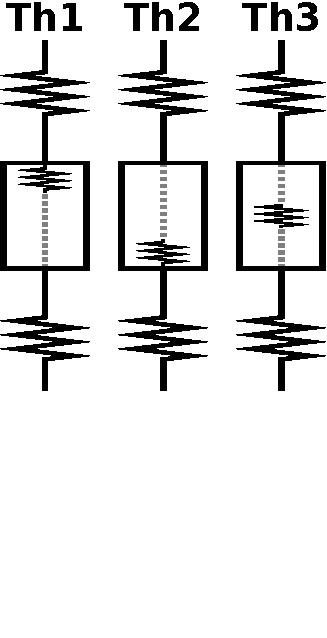
\includegraphics[width=0.26\columnwidth]{figures/mtmpi/th_multiple.pdf}
%     \label{fig:th_mode_mt}
%   }
%   \hspace{0.05\columnwidth}
%   % \vspace{-2.0ex}
%   \caption{Threading modes in MPI.  A line represents a thread; the
%     zigzag part represents an active thread in an OpenMP region; the
%     straight part represents a thread outside an OpenMP region; the
%     dotted part represents an idle thread in an OpenMP region; the
%     boxes represent MPI calls.}
%   \label{fig:th_modes}
%   % \vspace{-3.0ex}
% \end{figure}


\newsavebox\mpiOutsideBox
\begin{lrbox}{\mpiOutsideBox}
\begin{lstlisting}[linewidth=0.45\columnwidth]
#pragma omp parallel
{

  /* user computation */

}

MPI_Function();
\end{lstlisting}
\end{lrbox}

\newsavebox\mpiInsideMasterBox
\begin{lrbox}{\mpiInsideMasterBox}
\begin{lstlisting}[linewidth=0.45\columnwidth]
#pragma omp parallel
{
  /* user computation */
  #pragma omp master
  {
    MPI_Function();
  }
}
\end{lstlisting}
\end{lrbox}

\newsavebox\mpiInsideCriticalBox
\begin{lrbox}{\mpiInsideCriticalBox}
\begin{lstlisting}[linewidth=0.45\columnwidth]
#pragma omp parallel
{
  /* user computation */
  #pragma omp critical
  {
    MPI_Function();
  }
}
\end{lstlisting}
\end{lrbox}

\newsavebox\mpiInsideSingleBox
\begin{lrbox}{\mpiInsideSingleBox}
\begin{lstlisting}[linewidth=0.45\columnwidth]
#pragma omp parallel
{
  /* user computation */
  #pragma omp single
  {
    MPI_Function();
  }
}
\end{lstlisting}
\end{lrbox}

\begin{figure}%[h]
\setlength{\subfigcapskip}{5pt}
\centering
\subfigure[Outside a parallel region] {
  \usebox\mpiOutsideBox
  \label{fig:code_hybrid_outside}
}
\hfill
\subfigure[Inside omp \emp{master} region]{
  \usebox\mpiInsideMasterBox
  \label{fig:code_hybrid_master}
}
\\
\vspace{3.0ex}
\subfigure[Inside omp \emp{critical} region]{
  \usebox\mpiInsideCriticalBox
  \label{fig:code_hybrid_critical}
}
\hfill
\subfigure[Inside omp \emp{single} region] {
  \usebox\mpiInsideSingleBox
  \label{fig:code_hybrid_single}
}
\caption{Different use cases in hybrid MPI+OpenMP.}
\label{fig:code_omp}
\end{figure}

\begin{description}
\item[MPI\_THREAD\_SINGLE] \hfill \\
In this mode, only a single thread exists in every MPI process. This
model is commonly referred to as the MPI-only model, where multiple
MPI processes communicate with each other and no threads are involved.

\item[MPI\_THREAD\_FUNNELED] \hfill \\
In this mode, multiple threads can be created for parallelizing the
computation phases on every MPI process, but only the master thread is
allowed to access MPI stack. In an OpenMP program, this can be implemented
as either making MPI calls outside the OpenMP parallel region or protecting
the MPI calls with OpenMP master regions. Figure~\ref{fig:code_hybrid_outside}
and \ref{fig:code_hybrid_master} demonstrate those implementation
respectively.

\item[MPI\_THREAD\_SERIALIZED] \hfill \\
Similar as the funneled mode, multiple threads can be used to parallelize
the computation in the serialized mode. For the MPI communication phases,
however, any single thread can issue MPI calls at a time. That is, different
threads can concurrently perform the computation, but all of them need to
be synchronized in order to serialize the MPI calls.  In a typical OpenMP
program, this can be implemented by making MPI calls within OpenMP critical
regions or single regions as shown in Figure~\ref{fig:code_hybrid_critical}
and \ref{fig:code_hybrid_single} respectively.

\item[MPI\_THREAD\_MULTIPLE] \hfill \\
The multiple mode is different from the above levels, multiple threads
can concurrently perform both user computation and MPI communication.
The MPI implementation is required to provide appropriate synchronization
among threads (i.e., lock protection and memory barriers) to protect
accesses to shared internal data structures.

\end{description}


%%%%%%%%%%%%%%%%%%%%%%%%%%%%%%%%%%%%%%%%%%%%%%%%%%%%%%%%%%%%%%%%%%%%%%%%%%%%%
\section{MPI One-sided Communication}\label{sec:back-rma}
%%%%%%%%%%%%%%%%%%%%%%%%%%%%%%%%%%%%%%%%%%%%%%%%%%%%%%%%%%%%%%%%%%%%%%%%%%%%%

MPI-2 and MPI-3 introduced the MPI one-sided communication model
(also known as remote memory access or RMA). Unlike the well-known
two-sided communication (e.g., MPI\_Send\slash MPI\_Receive), the one-sided
mode allows applications to define more dynamic and data-driven communication
patterns where a process can directly access memory in another process
(i.e., window) through RMA operations such as \emp{put}, \emp{get} or
\emp{update}. Furthermore, all the operations are only issued from the
origin process, thus the program running on the remote process does not
need to call any MPI routines to match the operations. Figure~\ref{fig:back-rma}
demonstrates the difference between the two-sided mode and the one-sided mode.

\begin{figure}%[ht]
\centering
\subfigure[Two-Sided Mode.] {
  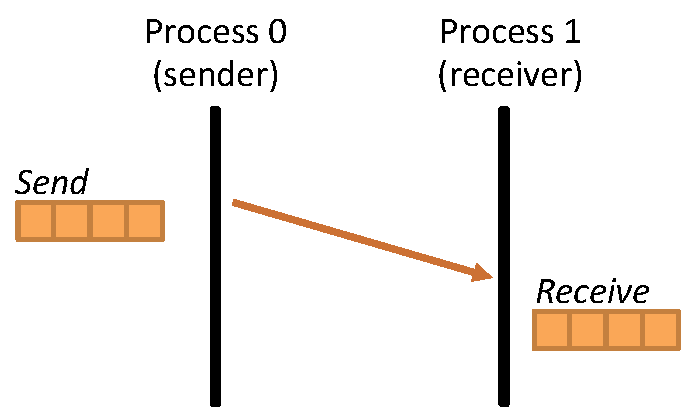
\includegraphics[height=0.28\textwidth]{figures/background/mode-rma-two-sided.pdf}
  \label{fig:back-rma-two-sided}
}
\hspace{-0.02\textwidth}
\subfigure[One-Sided Mode.] {
  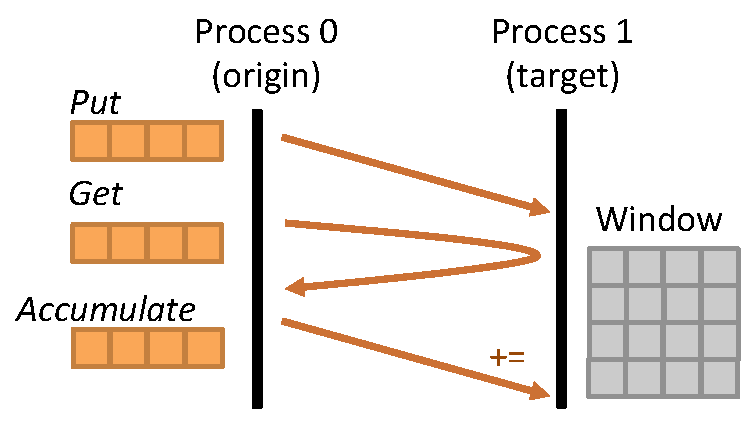
\includegraphics[height=0.28\textwidth]{figures/background/mode-rma-one-sided.pdf}
  \label{fig:back-rma-one-sided}
}
\caption{MPI Communication Modes}
\label{fig:back-rma}
\end{figure}


Because the second contribution of this thesis is a process-based asynchronous
progress model that comprehensively supports the strict MPI one-sided
communication semantics which is also the most challenging part in this work,
we then introduce the primary semantics of this communication mode in the rest
of this section. The semantics of the RMA communication can be divided into
following three primary steps: window creation, RMA synchronization and
issuing RMA operations.

%------------------------------
\subsection{Window Creation}
%------------------------------
A memory area on a process that is exposed to all other processes in a
specified group---allowing direct access to these processes---is called
a \emp{ window}. MPI-3 provides the following four window initialization
functions:

\begin{description}
\item[MPI\_Win\_create]\hfill \\
This routine exposes an RMA window for the memory region which is allocated
by user application in advance. The corresponding \fn{MPI\_Win\_free}
call only releases the RMA window, thus user is responsible for releasing
the memory region after window is freed.

\item[MPI\_Win\_allocate]\hfill \\
This routine allows MPI to internally allocate a memory region and expose
it to the other processes as a remotely accessible window. The corresponding
\fn{MPI\_Win\_free} call releases both the window structure and the memory
buffer.

\item[MPI\_Win\_allocate\_shared]\hfill \\
This routine allows MPI to initialize a shared window among processes
located in the same shared memory system (e.g., the same NUMA node) through
external system support such as mmap or XPMEM on Cray systems~\cite{xpmem}.
This shared memory region can be accessed by CPU load\slash store instructions
instead of MPI RMA operations, however, additional synchronization is required
to ensure the correctness with other concurrent RMA operations. The start
address of a remote window region mapped on the local process can be got from
the \fn{MPI\_Win\_shared\_query} call.

\item[MPI\_Win\_create\_dynamic]\hfill \\
This routine allows programs to expose an empty remote accessible window,
and then attach\slash detach one or multiple memory regions in later execution.
\end{description}

The above routines give user different levels of flexibility of window
creation. However, the routines with more flexibility also limit the possible
internal optimization can be provided from MPI implementations. For instance,
the most flexible \fn{MPI\_Win\_create\_dynamic} can rarely get any
optimization.

%------------------------------
\subsection{RMA Operations}
%------------------------------

After the remote accessible window is identified, a process can issue
\emp{put}, \emp{get}, or \emp{accumulate} operations to access this
window. Figure~\ref{fig:back-rma-one-sided} gives an image to demonstrate
data movement associated to those operations.

\begin{description}
\item[MPI\_Put]\hfill \\
This operation copies the data in the origin process's buffer to
the specified memory location in the window on the target process.

\item[MPI\_Get]\hfill \\
This operation copies data from the specified memory location
of remote window to the buffer located in the origin process's
local memory.

\item[MPI\_Accumulate]\hfill \\
This operation first transfers data from the origin process's buffer
to the target process, and then performs a update on the target side
following the user specified operation (e.g., \fn{MPI\_SUM}) and stores
the result into the window. We note that, unlike the put\slash get
operations, the accumulate operation is guaranteed to be \emp{ordered} and
\emp{atomic} per basic data element. We will introduce the ordering and
atomic semantics in Section~\ref{sec:back-rma-semantic}.
\end{description}

Beside above three basic RMA operations, there are three other
operations also defined in MPI standard: \fn{MPI\_Get\_accumulate},
\fn{MPI\_Fetch\_and\_op} and \fn{MPI}-\fn{\_Compare\_and\_swap}. The detailed
semantics of those operation can be found in~\cite{mpi30-report}.

%------------------------------
\subsection{RMA Synchronization}
%------------------------------

All the RMA operations are non-blocking MPI calls, which means the completion
of those data movement is not guaranteed at return. In addition, since processes
may concurrently access the same RMA window, we also need synchronization
among the involved processes in order to avoid any conflicts. MPI defines two
kinds of synchronization modes to handle those responsibilities in RMA communication,
they are the \emp{active mode} and the \emp{passive mode}. We introduce
each of them separately in this section.

\begin{figure}%[ht]
\centering
\subfigure[Fence.] {
  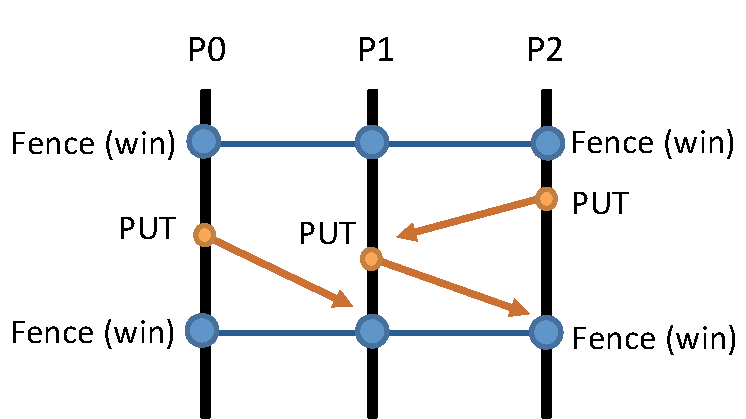
\includegraphics[height=0.25\textwidth]{figures/background/mode-rma-fence.pdf}
  \label{fig:back-rma-fence}
}
% \hspace{0.01\textwidth}
\subfigure[Post-Start-Complete-Wait.] {
  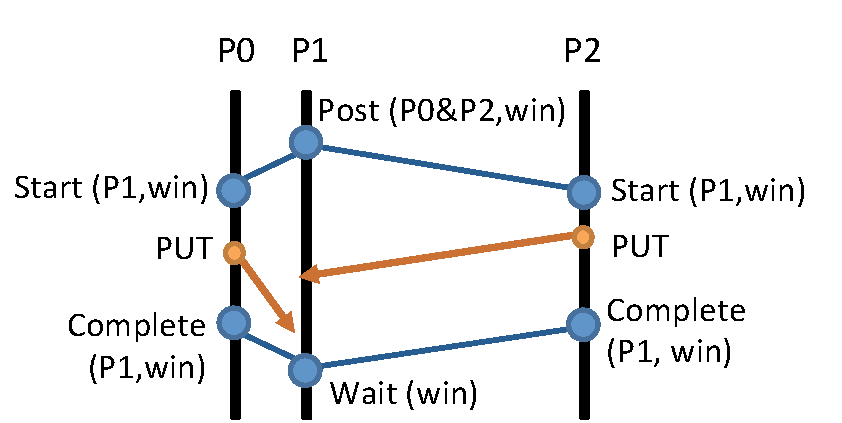
\includegraphics[height=0.25\textwidth]{figures/background/mode-rma-pscw.pdf}
  \label{fig:back-rma-pscw}
}
\\
\subfigure[Lock\_all-Unlock\_all.] {
  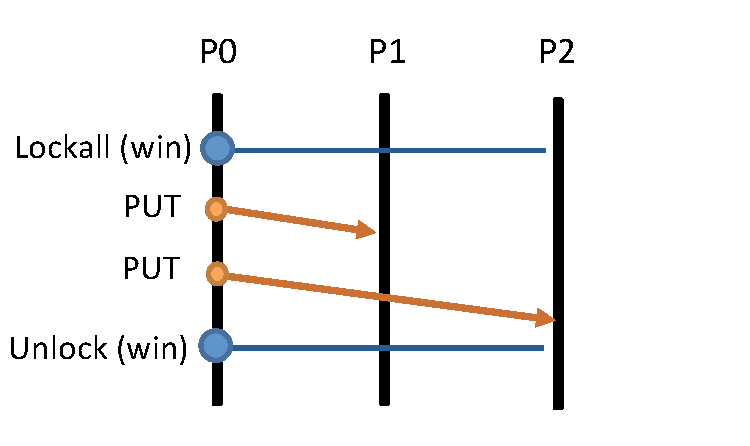
\includegraphics[height=0.26\textwidth]{figures/background/mode-rma-lockall.pdf}
  \label{fig:back-rma-lockall}
}
% \hspace{-0.06\textwidth}
\subfigure[Lock-Unlock.] {
  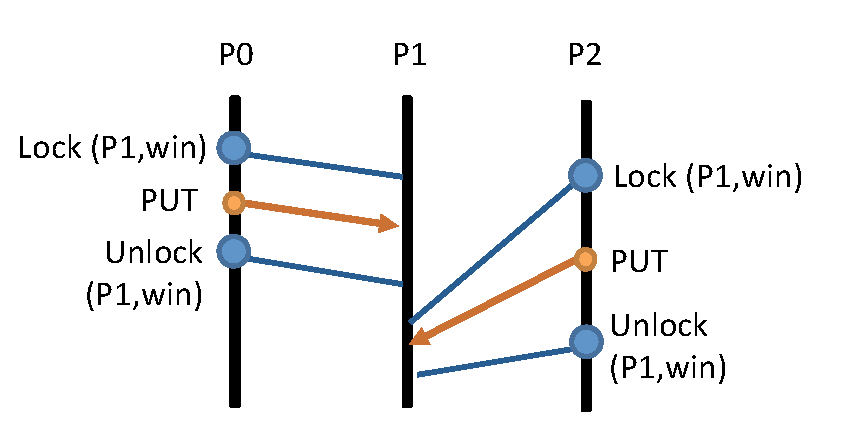
\includegraphics[height=0.26\textwidth]{figures/background/mode-rma-lock.pdf}
  \label{fig:back-rma-lock}
}
\caption{RMA Synchronization Modes}
\label{fig:back-rma-sync}
\end{figure}

\parahead{Active Mode}:
% \begin{description}
% \item[Active Mode]\hfill \\
This mode provides a similar synchronization as that in two-sided mode,
both the origin process and the target process need to explicitly
call the synchronization. Two sets of synchronization calls are defined
in MPI: \emp{fence} and \emp{post-start-complete-wait}.

\begin{itemize}
  \item In \emp{fence} synchronization, all the processes in the window
  must collectively call \fn{MPI\_Win\_Fence} routine to synchronize with
  each other (Figure~\ref{fig:back-rma-fence}) similar as \emp{barrier} in the
  two-sided communication mode. The return from the fence call guarantees:
  (1) all the processes have arrived at the fence call; (2) all the outstanding
  RMA operations and local load\slash store instructions issued on this window
  have been completed.

  \item The \emp{post-start-complete-wait} synchronization can be considered as
  a subset of fence (Figure~\ref{fig:back-rma-pscw}). At the beginning of
  the RMA communication, the target process (P1) calls \fn{MPI\_Win\_post}
  to expose its window to one or several processes and the origin process
  (P0 or P2) performs \fn{MPI\_Win\_start} to match the post call and then
  starts the remote access; at the end of the communication, the origin
  process needs to call \fn{MPI\_Win\_complete} to complete its operations
  and the target process needs to call \fn{MPI\_Win\_wait} to ensure all
  the operations issued on its window have been finished.
\end{itemize}

\parahead{Passive Mode}:
% \item[Passive Mode]\hfill \\
Apart from the semi-dynamic active mode, MPI also offers the passive mode
which performs completely dynamic pattern. That is, only the process
issuing operations (origin process) is required to explicitly call the
synchronization. Two sets of synchronization calls are defined:
\emp{lock\_all-unlock\_all} and \emp{lock-unlock}.

\begin{itemize}
  \item The \emp{lock\_all} serial provides global synchronization similar
  as the \emp{fence}, however, only the origin process (e.g., P0 in
  Figure~\ref{fig:back-rma-lockall}) issues the \fn{MPI\_Win}-\fn{\_lock\_all}
  and \fn{MPI\_Win\_unlock\_all} calls. The return from \emp{lock\_all}
  ensures the origin process have acquired the \emp{shared} lock on all
  the other processes, and the return from \emp{unlock\_all} ensures:
  (1) the locks have been released, and (2) all the operations issued from
  this process have been completed remotely.

  \item The \emp{lock} serial can be also considered as a subset of \emp{lock\_all}
  which provides per-target exclusive\slash shared lock (\fn{MPI\_LOCK\_EXCLUSIVE}
  or \fn{MPI\_LOCK\_SH}-\fn{ARED} lock type). We note that two origin processes can
  concurrently acquire a \emp{shared} lock on the same target window, however,
  any other lock requests must be serialized with the \emp{exclusive} lock.
  Figure~\ref{fig:back-rma-lock} shows an example. Simultaneous \emp{lock\_all}
  and \emp{lock} follow the same rule.

  \item Besides the lock calls, the passive mode also offers two \emp{flush}
  synchronization routines that only complete the outstanding RMA operations,
  and a \emp{sync} routine (\fn{MPI\_Win\_sync}) that synchronizes the data
  of its local window updated by remote RMA operations and the one updated
  by load\slash store instructions. \fn{MPI\_Win\_flush} completes the operations
  issued from the origin process to a single target process, and \fn{MPI\_Win\_flush\_all}
  completes operations issued from the origin process to any target processes
  in the window.
\end{itemize}

% \end{description}

%------------------------------
\subsection{Ordering and Atomicity}\label{sec:back-rma-semantic}
%------------------------------

In the section, we introduce the ordering and atomicity semantics
guaranteed for \emp{accumulate}-like operations (i.e., \emp{accumulate},
\emp{get\_accumulate}, \emp{fetch\_and\_op}, \emp{compare\_and\_swap})
in MPI standard by using two examples for each.

Any MPI implementation must guarantee the ordering between accumulate-like
operations that are issued from the same origin process and sent to the
same target. Figure~\ref{fig:code_rma_ordering} gives an example.

\newsavebox\mpiRmaOrdering
\begin{lrbox}{\mpiRmaOrdering}
\begin{lstlisting}[linewidth=0.7\columnwidth]
P0                              P1
                                x = 2;
Lock(P1, win);
Get_accumualte(x, y, +1, P1);
Accumualte(x, +2, P1);
Unlock(P1, win);
Read y;
\end{lstlisting}
\end{lrbox}

\begin{figure}[ht]
\centering
\vspace{2.0ex}
\usebox\mpiRmaOrdering
\caption{Example of Ordering Semantics in MPI RMA communication.}
\label{fig:code_rma_ordering}
\end{figure}

MPI also guarantees the atomicity of any accumulate-like operations
that are issued to the same target process and the same window memory
location per basic data element (e.g., integer or double, but any
MPI derived datatype is not included). The operations can be issued
from the same origin process or from different ones.
Figure~\ref{fig:code_rma_atomic} gives an example.


\newsavebox\mpiRmaAtomic
\begin{lrbox}{\mpiRmaAtomic}
\begin{lstlisting}[linewidth=1\columnwidth]
P0                      P1                      P2
                                                x = 2;
Lock(SHARED, P2, win);  Lock(SHARED, P2, win);
Accumualte(x, +1, P1);
                        Accumualte(x, +2, P1);
Unlock(P2, win);        Unlock(P2, win);
\end{lstlisting}
\end{lrbox}

\begin{figure}[ht]
\centering
\vspace{2.0ex}
\usebox\mpiRmaAtomic
\caption{Example of Atomicity Semantics in MPI RMA communication.}
\label{fig:code_rma_atomic}
\end{figure}